\def\unit{1cm}

\def\RadiusVec{0.2}
\tikzset{
   pics/.cd,
   vector out/.style={
      code={
         \draw[#1] (0,0)  circle (\RadiusVec) (45:\RadiusVec) -- (225:\RadiusVec) (135:\RadiusVec) -- (315:\RadiusVec);
      }%end code   
   }%end style
}%end tikzset
\tikzset{
   pics/.cd,
   vector in/.style={
      code={
        \draw[#1] (0,0)  circle (\RadiusVec);
        \fill[#1] (0,0)  circle (.05);
      }%end code   
   }%end style
}%end tikzset


    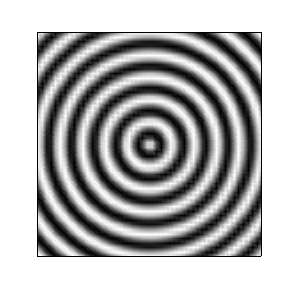
\begin{tikzpicture}
      \centering

      \def\Sample{50} %Résolution de la figure

      \begin{scope}[xshift=11cm,scale=0.5]
         \begin{axis}[
            xlabel={},
            ylabel={},
            xticklabels={,,},
            yticklabels={,,},
            view={0}{90},
            colormap/blackwhite,
            ytick style={draw=none},
            xtick style={draw=none},
            axis equal image
            ]

            \addplot3 [surf, shader=interp, samples = \Sample, domain=0:10, y domain = 0:10] {cos(deg(2*pi*sqrt((x-5)^2+(y-5)^2)/1))};

         \end{axis}


      \end{scope}

    \end{tikzpicture}
